\documentclass[preview,border=0mm,convert={density=600,outext=.png}]{standalone}
\usepackage{amsfonts,amssymb,amsmath}
\usepackage{tikz}
\usetikzlibrary{automata,shapes,patterns,calc,arrows}
\usepackage{xspace}
\usetikzlibrary{arrows}
\usetikzlibrary{automata}
\usetikzlibrary{shapes,snakes}
\usetikzlibrary{calc}
\usetikzlibrary{patterns}
\usetikzlibrary{shapes.geometric}
\usetikzlibrary{positioning}
\tikzstyle{action}=[rounded corners=.5,minimum size=.4cm,draw=gray!90,inner sep=1pt,fill=gray!20,very thick]
\tikzstyle{every edge}=[draw,>=stealth',shorten >=1pt]

%\tikzset{node distance=2.5cm}
%\tikzset{every node/.style={anchor=base}}

%% edges
\tikzset{>=latex,bend angle=20}
\tikzstyle{line}=[line width=.6pt]
\tikzstyle{arrow}=[->,line]
\tikzstyle{dblarrow}=[<->,line]
\tikzstyle{invarrow}=[<-,line]
\tikzstyle{initial}=[invarrow]
\tikzset{selfloop/.style={arrow,out={#1-30},in={#1+30},looseness=6}}
% we use tikzset here because tikzstyle does not allow arguments
 

\begin{document}

\centering
  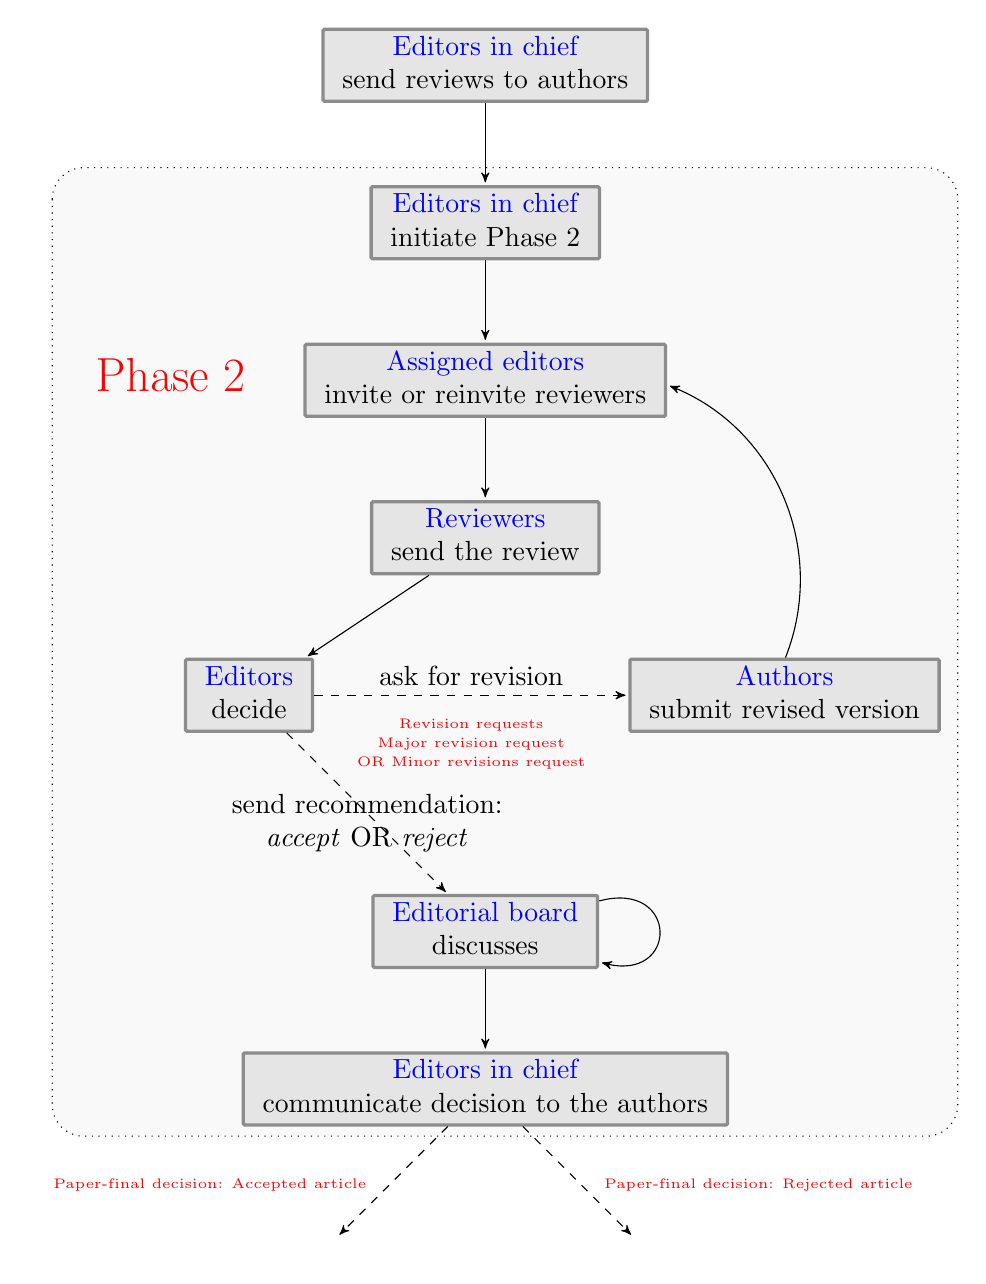
\begin{tikzpicture}[scale=1]
    \draw[dotted,rounded corners=4mm,fill=gray!5]
    ($(-3.5,-1.3)$) rectangle ($(8,-13.6)$) ;

    \node[action] (sendreviews) at (2,0) {\begin{tabular}{c}\textcolor{blue}{Editors in chief}\\ send reviews to authors\end{tabular}};
    \node[action] (movephase2) at (2,-2) {\begin{tabular}{c}\textcolor{blue}{Editors in chief}\\ initiate Phase 2\end{tabular}};
    \node[action] (invitereviewers) at (2,-4) {\begin{tabular}{c}\textcolor{blue}{Assigned editors}\\ invite or reinvite reviewers\end{tabular}};
%    \node[action] (answerinvitation) at (2,-7) {\begin{tabular}{c}\textcolor{blue}{Reviewers}\\ answer the review request \end{tabular}};
    \node[action] (sendreview) at (2,-6) {\begin{tabular}{c}\textcolor{blue}{Reviewers}\\ send the review\end{tabular}};
    \node[action] (submitrevised) at (5.8,-8) {\begin{tabular}{c}\textcolor{blue}{Authors}\\ submit revised version\end{tabular}};
    \node[action] (recommendation) at (-1,-8) {\begin{tabular}{c}\textcolor{blue}{Editors}\\ decide\end{tabular}};
%    \node[action] (weeklydigest) at (5.8,-14.5) {\begin{tabular}{c}\textcolor{blue}{Weekly digest}\\ informs editorial board\end{tabular}};
    \node[action] (discusses) at (2,-11) {\begin{tabular}{c}\textcolor{blue}{Editorial board}\\ discusses\end{tabular}};
    \node[action] (communicatedecision) at (2,-13) {\begin{tabular}{c}\textcolor{blue}{Editors in chief}\\ communicate decision to the authors\end{tabular}};
    \node (accept) at (0,-15) {\ };
    \node (reject) at (4,-15) {\ };
    
    \node (unnamed) at (-2,-4) {\begin{tabular}{c}\textcolor{red}{\LARGE{Phase 2}}\end{tabular}};
  
    \draw[->] (sendreviews) edge (movephase2) ;
    \draw[->] (movephase2) edge (invitereviewers) ;
    \draw[->] (invitereviewers) edge (sendreview) ;
%    \draw[dashed, ->] (answerinvitation) edge node {\begin{tabular}{c}\tiny{\color{red} Accepted reviewer invitation}\end{tabular}} (sendreview) ;
%    \draw[dashed, ->] (answerinvitation) edge[bend right=30] node[above] {\begin{tabular}{c}\tiny{\color{red} Refused reviewer invitation}\end{tabular}} (invitereviewers) ;
    \draw[->] (sendreview) edge (recommendation) ;
    \draw[dashed, ->] (recommendation) edge node[below] {\begin{tabular}{c}\tiny{\color{red} Revision requests}\\[-.5em] \tiny{\color{red}Major revision request}\\[-.5em] \tiny{\color{red}OR Minor revisions request}\end{tabular}} node[above] {ask for revision} (submitrevised) ;
	\draw[dashed, ->] (recommendation) edge node {\begin{tabular}{c}\ \\[-.5em] send recommendation:\\ \textit{accept} OR \textit{reject}\end{tabular}} (discusses) ;
%    \draw[dashed, ->] (recommendation) edge[bend right=20] (weeklydigest) ;
%    \draw[->] (weeklydigest) edge (discusses) ;
    \draw[->] (discusses) edge [distance = 30, in = 0, out = 0, loop right] (discusses) ;
    \draw[->] (discusses) edge (communicatedecision) ;
    \draw[dashed, ->] (communicatedecision) edge node[left] {\begin{tabular}{c}\tiny{\color{red} Paper-final decision: Accepted article}\end{tabular}} (accept) ;
    \draw[dashed, ->] (communicatedecision) edge node[right] {\begin{tabular}{c}\tiny{\color{red} Paper-final decision: Rejected article}\end{tabular}} (reject) ;
%    \draw[dashed, ->] (submitrevised) edge node {\begin{tabular}{c}\tiny{\color{red} Reviewer assignment to a new version of an article}\\ if ``automatically reinvite reviewers''\end{tabular}} (sendreview) ;
    \draw[->] (submitrevised) edge[bend right=45] (invitereviewers) ;
  \end{tikzpicture}

\end{document}